% !TEX root = ../main.tex

\chapter{Kerr black hole} % Main chapter title
\label{Chapter2}

%----------------------------------------------------------------------------------------

\section{General Relativity}

General Relativity is the theory of space, time and gravitation developed by Einstein in 1915. 
It introduces a new viewpoint on gravity and its relation with the fabric of spacetime, a \emph{manifold} that bounds our three spatial dimensions with time.
The concept challenged our deeply ingrained and intuitive notions of nature, partially because the mathematical background needed to understand the precise formulation of the theory was unfamiliar to much of the physics community at the time.
This formulation corresponds to a field theory with the dynamical object of study being the metric of spacetime, $\bm{g}=g_{\mu\nu} \dd x^\mu \dd x^\nu$, connecting geometry with mass and energy through Einstein's field equations.
The theory inherits diffeomorphism invariance, \emph{i.e.} remains the same theory by an active change of coordinates, which was at the core of definition of manifolds.

Immediately after, in 1916, Schwarzschild found the first solution \cite{Schwarzschild1916}, describing a static spherical isolated object.
Then, the theory was left aside because of the numerous coupled nonlinear equations, but the astronomical discovery of compact and highly energetic objects in the 1950s breaded new interest into the somewhat dormant GR, mainly because it was thought that these quasars and compact X-ray sources had suffered some form of gravitational collapse or that strong gravitational fields were present.
Soon after, the modern theory of gravitational collapse was developed in the mid-1960s, including other BH solutions, for example Kerr's \cite{Kerr1963}.

The theory of GR can be elegantly described in the form of the Hilbert action,
\begin{align}
    S_{H} = \frac{1}{16\pi} \int \dd^4 x \sqrt{-g} \,R ~,
    \label{eq2:actionGR}
\end{align}
where $g=\det(g_{\mu\nu})$ and $R=g_{\alpha\beta} R^{\alpha\beta}$ corresponds to the Ricci scalar.
Naturally, the first solutions corresponded to pure gravity, usually designated as vacuum solutions \cite{Wald2010}, which obey
\begin{align}
    R_{\mu\nu} = 0 ~.
    \label{eq2:vacuumGR}
\end{align}
Despite their simplicity, they enjoy some very fascinating nontrivial properties. 
One of which is the existence of an event horizon, a surface that separates two causally disconnected regions of spacetime.

The underlying technique behind the study of superradiance is the linearization of Einstein and/or Maxwell equations around known BHs in stationary equilibrium.
These perturbations will obey a series of partial differential equations whose dynamical variables are components of the Weyl tensor, $C_{\mu\nu\rho\sigma}$, or the Maxwell field tensor, $F_{\mu\nu}$.
Thanks to the NP formalism we will be able to decouple and separate the equations for both GWs and EM waves, revealing decoupled variables which contain all the information needed about the nontrivial perturbations, instead of working with all components of the field tensors.

For the gravitational case, a straightforward way of obtaining a linearized theory is to consider a background stationary BH solution, $g_{\mu\nu}{}^B$, and then expanding the field equations \eref{eq2:vacuumGR} using the metric 
\begin{align}
    g_{\mu\nu} = g_{\mu\nu}{}^B + h_{\mu\nu}{}^P ~,
    \label{eq2:metricBP}
\end{align}
keeping only terms that are $\mathscr{O}(h_{\mu\nu}{}^B)$. The indices $B$ and $P$ refer to the background and perturbations, respectively.
As a result we are left with a wave equation in the given background. 

In this work we will focus on (massless, neutral) electromagnetic waves and perturbations are performed including EM interactions through the Maxwell action
\begin{align}
    S_{EM} = - \frac{1}{4} \int \dd^4 x \sqrt{-g} \,F_{\alpha\beta} F^{\alpha\beta} ~,
     \label{eq2:actionEM}
\end{align}
where $F_{\mu\nu}$ is the Maxwell tensor.
Variation of both actions, $\delta(S_H + S_{EM}) = 0$, result in two field equations
\begin{align}
    \nabla_\mu F^{\mu\nu} &= 0 ~, \label{eq2:maxwellEM} \\
    R_{\mu\nu} - \frac{R}{2} g_{\mu\nu} &= 8 \pi T_{\mu\nu} \label{eq2:EM+GR}  ~.
\end{align}
The first equation is just the usual of Maxwell equation in curved spacetime.
The latter are the Einstein field equations, reflecting the backreaction of the electromagnetic waves into the geometry through the presence of the EM stress-energy tensor
\begin{align}
    T_{\mu\nu} = F_{\mu\alpha} F_{\nu}{}^{\alpha} - \frac{1}{4} g_{\mu\nu} F^2  ~.
    \label{eq2:stressenergyEM}
\end{align}
These equations completely describe the system, but the problem is analytically untreatable, so we will resort to perturbation theory, considering the field $A^\mu$ to be small. 
This is a very good approximation, as the gravitational field near a stellar-mass BHs is considerably stronger then the radiation emitted by nearby astrophysical sources.
As the stress-energy tensor is quadratic in the fields, $T_{\mu\nu}\sim\mathscr{O}(A^2)$, then we can ignore the backreaction and the field equations for the metric $g_{\mu\nu}$ reduce to \eqref{eq2:vacuumGR}.

%----------------------------------------------------------------------------------------

\section{Spacetime symmetries}

It was generally accepted that a perfectly spherical symmetrical star would collapse to a Schwarzschild BH, although at the time the effect of a slightest amount of angular momentum on a gravitational collapse was not known.
Finding a metric with intrinsic rotation could give insight into such a problem. Due to the lack of spherical symmetry, the problem became much harder, and took roughly 50 years after Schwarzschild's discovery to find a metric for a rotating body.
Imposing symmetries to the final metric was essential to solve the field equations.

If we represent our spacetime and corresponding fields by $(\mathscr{M}, g_{\mu\nu}, \psi)$, then the pullback $f^*$ of the diffeomorphism $f:\mathscr{M}\rightarrow\mathscr{M}$ would give us the same physical system $(\mathscr{M}, f^* g_{\mu\nu}, f^* \psi)$.
Since diffeomorphisms are just active coordinate transformations, such concept may raise some confusion, as we do not seem to obtain any new information to work with. 
Almost all physical theories are coordinate invariant, as is Newtonian mechanics and Special Relativity, but in such theories there is a preferable coordinate system, while the same does not hold true for GR.
An analogy can be made with the path integral formalism in QFT, where special consideration is taken when summing all field configurations in order to not overcount indistinguishable configurations, as is the case of gauge field theories.
A similar ambiguity can occur in GR, where two apparently different solutions can be related by a diffeomorphism and are actually ``the same'', so we must be careful when deriving and analyzing any geometries.

Despite the added complexity of Einstein's field equations, it is still possible to find exact nontrivial solutions in a systematic way by considering spacetimes with symmetries with the use of Killing vector fields.
A vector field $\bm{\xi}$ that obeys
\begin{align}
    \left(\mathscr{L}_{\bm{\xi}} \,\bm{g} \right)_{\mu\nu} = 0  
    \label{eq2:killing}
\end{align}
is called a Killing field. Locally, this expression reduces to $\nabla_\mu \xi_\nu + \nabla_\nu \xi_\mu = 0$.

A \emph{stationary} solution implies the existence of a Killing vector $\bm{k}$ that is asymptotically timelike, $\bm{k}^2>0$, therefore allowing us to normalize our vector such that $\bm{k}^2 \rightarrow 1$. 
Unlike the case of the static spacetime, a stationary metric does not show invariance under reversal of the time coordinate, which is natural considering a system with angular momentum. 
Futhermore, a solution is also \emph{axisymmetric} if there is an asymptotically spacelike Killing field $\bm{m}$ whose integral curves are closed.
A solution is stationary and axisymmetric if both symmetries are present, along with commuting fields, $[\bm{k} , \bm{m}] = 0$, \emph{i.e.} rotations about the axis of symmetry commute with time translations \cite{Wald2010}. The commutativity of the fields implies the existence of a set of coordinates, $(t,r,\theta,\varphi)$, such that
\begin{align}
    \bm{k} = \frac{\partial}{\partial t} ~, \qquad \bm{m} = \frac{\partial}{\partial \varphi} ~.
    \label{eq2:tPhiKilling}
\end{align}
As a direct implication of this choice of chart, components of the metric stay independent of $(t,\varphi)$, in virtue of \eqref{eq2:killing},
\begin{align}
    \left(\mathscr{L}_{\bm{m}} \,\bm{g} \right)_{\mu\nu} = \frac{\partial g_{\mu\nu}}{\partial \varphi} = 0 ~,
    \label{eq2:lieMetricTPhi}
\end{align}
with the same holding true for $\bm{k}$, hence we can write $g_{\mu\nu} = g_{\mu\nu}(r,\theta)$. 

One of the major applications of Killing vectors is to find conserved charges associated with the motion along a geodesic spanned by the field.
These quantities are defined by taking the geodesics to regions of space that are asymptotical flat, where the geometry does not affect the observer.
In the case of the Kerr solution, we have two Killing vectors, $\bm{k}$ and $\bm{m}$, which are naturally associated with the total mass $M$ and angular momentum $J$ of the BH, respectively.
This is usually done by evaluating the Komar integrals \cite{Heusler1996, Townsend1997}, which can be written in a covariant way as
\begin{align}
    M = \frac{1}{8 \pi} \int_{S^2_\infty} \star \dd \bm{k}^\flat  =  -\frac{1}{4}& \lim_{r\to\infty}  \int_0^\pi \dd\theta \sqrt{-g} \, g^{t\alpha} g^{r\beta} g_{t[\alpha,\beta]} ~, \label{eq2:komarMass} \\
    J = -\frac{1}{16 \pi} \int_{S^2_\infty} \star \dd \bm{m}^\flat = \frac{1}{8}& \lim_{r\to\infty}  \int_0^\pi \dd\theta \sqrt{-g} \, g^{t\alpha} g^{r\beta} g_{\varphi[\alpha,\beta]} ~, \label{eq2:komarSpin}
\end{align}
where the usual notation $\bm{k}^\flat \equiv g_{\mu\nu} k^\mu \dd x^\nu$ transforms a vector into a one-form and the operator $\star : \Omega^{p}(\mathscr{M})\to\Omega^{4-p}(\mathscr{M})$ is the Hodge dual map for $p$-forms.
In order to complete the integration in the last step are assumed \eref{eq2:tPhiKilling} and \eref{eq2:lieMetricTPhi}, keeping $(t,r)$ constant. 
According to the widely accepted \emph{no-hair conjecture} \cite{Carter1971}, these two quantities completely define a stationary (neutral) BH. 

%----------------------------------------------------------------------------------------

\section{Kerr-Schild coordinates}

Naturally, Kerr was not the only one looking for such solution.
Many presented other geometries to approximately describe a rotating star. 
Most of the solutions were one-parameter modifications to Schwarzschild that were not asymptotically flat. 
Simply using stationary and axisymmetric symmetries and then solving Einstein equations clearly did not suffice.

Kerr's success originated in of Petrov's classification of spacetimes, which used the algebraic properties of the Weyl tensor to distinguish the solutions in 3 types, with some subcases.
He assumed that his solution would have the same classification as Schwarzschild's, associated with the geometry of isolated central objects, such as stars and BHs. 
From this assumption, using GR spinor techniques and only then imposing the Killing vectors in \eqref{eq2:tPhiKilling} was possible to find a new solution. 
Kerr's metric appear in his original paper \cite{Kerr1963} in the form
\begin{align}
    \begin{split}
        \bm{g} = & \left(1 - \frac{2 M r}{\rho^2} \right) (\dd v - a \sin^2\theta \dd \chi )^2 \\
        & - 2  (\dd v - a \sin^2\theta \dd \chi )  (\dd r - a \sin^2\theta \dd \chi ) \\
        & - \rho^2 (\dd \theta^2 + \sin^2\theta \dd \chi^2 ) ~,
    \end{split}
    \label{eq2:KerrIngoingEF}
\end{align}
where $a$ is a parameter, $M$ is the BH mass and $\rho^2 = r^2 + a^2 \cos^2\theta$. Naturally the time Killing vector is $\partial_v$ and $\partial_\chi$ is the axial field, entailing that $J = a M$.

Taking the limit of $a\to0$, we reduce the metric to the Schwarzschild solution in ingoing Eddington-Finkelstein (EF) coordinates, $(v,r,\theta,\chi)$, which are useful to study ingoing (to the horizon) geodesics and remove the horizon coordinate singularity.
When a given metric has singularities it is not trivial to identify if they are physical singularities or an artifact resultant of choice of chart, removable by a better choice of coordinates. 
That being said, this raises the difficulty of finding the essential singularities.
The best way to look for these singularities is to compute curvature scalar quantities, and if they diverge in one particular chart, then they diverge in all charts.
Since any BH is just a vacuum solution, then the Ricci scalar vanishes, $R=0$, so we resort to the Kretschmann scalar,
\begin{align}
    \label{eq2:KerrKretschmann}
    R_{\alpha\beta\gamma\delta} R^{\alpha\beta\gamma\delta} = \frac{48 M (r^2 - a^2\cos^2\theta) \left[ (r^2 - a^2\cos^2\theta) ^2 - 16 r^2 M^2 a^2\cos^2\theta \right] }{(r^2 + a^2\cos^2\theta)^6} ~,
\end{align}
that clearly diverges for $\rho^2=0$.
The Schwarzschild singularity, $r=0$, is replaced with the Kerr singularity $(r,\theta)=(0,\pi/2)$.
It is not clear what is the geometry of the Kerr singularity if we interpret $r$ and $\theta$ as being part of the ordinary spherical coordinates.
Although the metric is singular, we can draw some insight considering $(r,\theta)$ constant and then the limit of $r\to0$ through the equatorial plane,
\begin{align}
    \label{eq2:KerrSingularity}
    {\bm{g}}\rvert_{\mathrm{singularity}} \sim \dd v^2 - a^2 \dd \chi^2 ~.
\end{align}
Hence the metric is reduced to the line element of the circle, $S^1$, confirming a \emph{ring singularity} of radius $a$.
This result implies that we may only reach the singularity, $\rho^2=0$, by approaching the Kerr BH through the equatorial plane. 

The Kerr-Schild theory provides the ``cartesian'' form \cite{Teukolsky2015}, 
\begin{align}
    \label{eq2:KerrSchild}
    \begin{split}
        \bm{g} = & \, \dd \tilde{t}^2 - \dd x^2 - \dd y^2 - \dd z^2 \\
        & - \frac{2 M r^3}{r^4 + a^2 z^2} \left[ \dd \tilde{t} + \frac{r (x \dd x + y \dd y) + a ( y \dd x - x \dd y)}{r^2+a^2} + \frac{z}{r} \dd z \right]^2 ~,
    \end{split}
\end{align}
which is particularly useful to understand the singularity geometry.
In this metric, $r$ is no longer a coordinate but a function of this chart coordinates $(\tilde{t},x,y,z)$.
We can relate the The Kerr-Schild metric to the original Kerr solution, using
\begin{align}
    \label{eq2:InEFtoKSchild}
    \tilde{t} = v - r ~, \qquad x+ i y = (r -i a) e^{i \chi} \sin\theta ~,\qquad z=r\cos\theta ~,
\end{align}
which implies that $r(x,y,z)$ is implicitly given by
\begin{align}
    \label{eq2:rConditionKSchild}
    r^4 - (x^2+y^2+z^2-a^2)r^2 -a^2 z^2 = 0 ~.
\end{align}
This condition deserves a more in-depth analysis.
For increasing $r$, the surfaces obeying \eqref{eq2:rConditionKSchild} approximates perfect spheres as the geometry gets more and more flat.
Minkowsky flat space is immediately also guaranteed for $M=0$.
On the other hand, as we approach the singularity on $z=0$ and $x^2+y^2 = a^2$, rotation effects deform the surfaces into oblate spheroids ($\theta\ne\pi/2$ for the strict inequality).
Such remarks are visually demonstrated in~\fref{fig2:kerrchild}.

\begin{figure}[h]
    \centering
    \begin{subfigure}[c]{0.45\textwidth}
        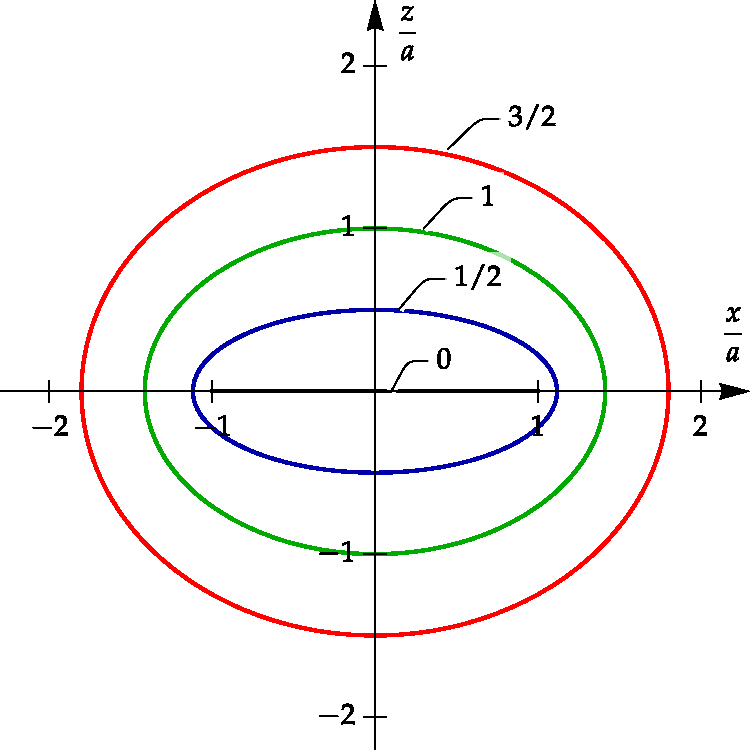
\includegraphics[width=\textwidth]{kerrchild2d}
    \end{subfigure}
    \hspace{1cm}
    \begin{subfigure}[c]{0.35\textwidth}
        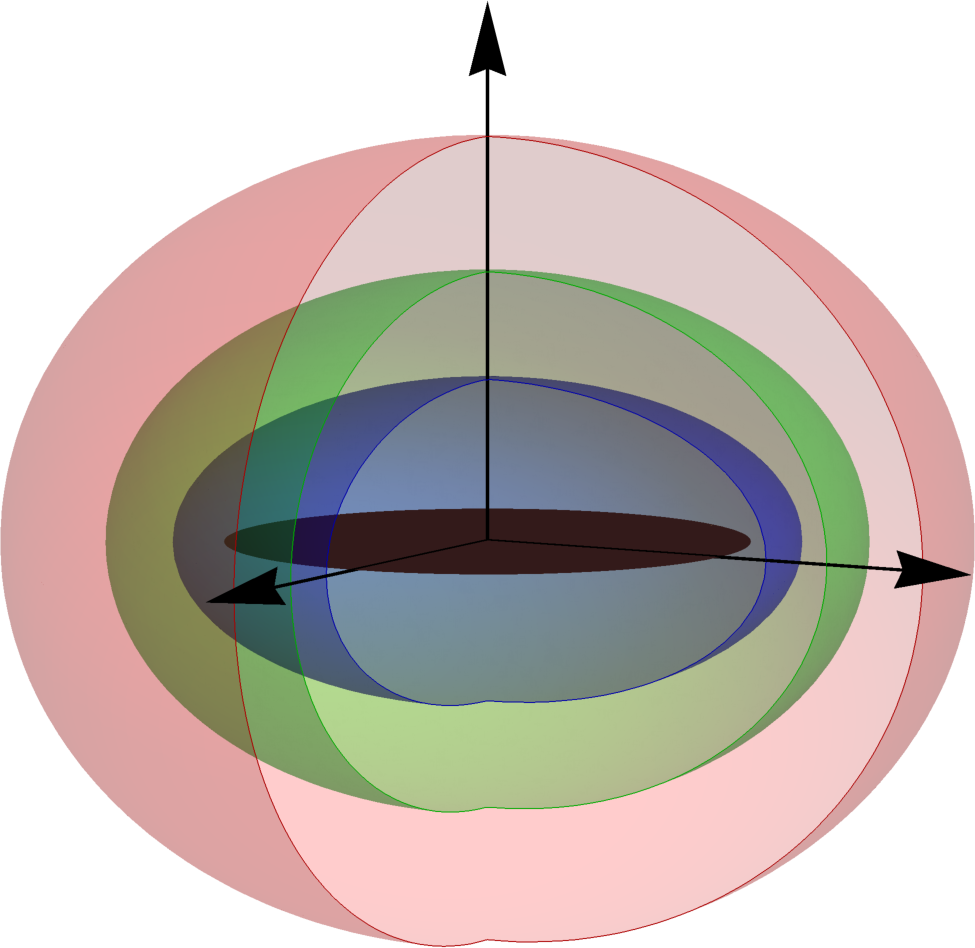
\includegraphics[width=\textwidth]{kerrchild3d}
    \end{subfigure}
    \caption{Contour plots of the surface $r(x,y,z)/a$ for constant values of $0,\,1/2,\,1,\,3/2$, in the Kerr-Schild coordinates. The left plot is the intersection of the $y=0$ plane with the 3D representation (right) that spotlights the ring singularity. Dashed curves representing orthogonal constant $\theta(x,y,z)$ hypersufaces become asymptotically affine.}\label{fig2:kerrchild}
\end{figure}

Even though the Kerr-Schild metric takes $r>0$ values, there is no mathematical reason to restrict $r$ strictly to positive values.
Thus, hypersurfaces of constant $r$ can also be represented by $-r$. 
This means that this chart can be analytically extended to regions where $r<0$.
It is possible to obtain a \emph{maximally extended} solution by analytic continuation and a proper collage of charts \cite{Townsend1997}.
This gives mathematical access to new spacetime regions, even tough most of them show unphysical properties.

%----------------------------------------------------------------------------------------

\section{Boyer-Linquist coordinates}

Considering the problem in hand, the most suitable coordinates for work with the Newman-Penrose (NP) formalism, are the Boyer-Linquist (BL) coordinates \cite{Boyer1967},
\begin{align}
    \label{eq2:KerrBL}
    \begin{split}
        \bm{g} = & \left(1 - \frac{2 M r}{\rho^2} \right) \dd t^2 + 2 a \sin^2\theta \frac{(r^2+a^2-\Delta)}{\rho^2} \dd t \dd \varphi \\
        &- \frac{(r^2+a^2)^2- \Delta a^2 \sin^2\theta}{\rho^2} \sin^2\theta \dd\varphi^2 - \frac{\rho^2}{\Delta} \dd r^2 - \rho^2 \dd \theta^2 ~,
    \end{split}
\end{align}
where we define $\Delta=r^2-2 M r + a^2$.
In order to show that these correspond to the same solution, the change of coordinates
\begin{align}
    \label{eq2:InEFtoBL}
    \dd v = \dd ( t + r_* ) ~, \qquad \dd \chi = \dd \varphi + \frac{a}{\Delta} \,\dd r ~,
\end{align}
takes us back to the original Kerr form \eref{eq2:KerrIngoingEF}.
The coordinate $v$ is given by the known ingoing EF transformation, defined by the Regge-Wheeler coordinate, also named \emph{tortoise} coordinate, which is very useful to construct null directions.
In the case of the Kerr BL metric, it holds that
\begin{align}
    \label{eq2:tortoise}
    \frac{\dd r_*}{\dd r} = \frac{r^2+a^2}{\Delta} ~.
\end{align}
These coordinates are usually referred as ``Schwarzschild like'', as they lead to the spherical static case in standard curvature coordinates when setting $a=0$. 
Time inversion symmetry is characteristic of the static Schwarzschild spacetime, but the same does not hold for Kerr's.
Nevertheless, this specific form is invariant under the inversion $(t,\varphi)\to(-t,-\varphi)$, also known as the \emph{circular condition}, an intuitive notion from physical systems with angular momentum \cite{Wald2010, Heusler1996}.
This discrete symmetry eliminates most of the off-diagonal components of the BL metric, $g_{tr} = g_{\varphi r} = g_{t \theta} = g_{\varphi \theta} = 0$, making it the simplest to perform calculations.

To study the possible horizons of the Kerr BH, we will consider $\bm{n} = (\dd r)^\sharp \equiv (g^{\mu\nu} \nabla_\nu r) \partial_\mu$ which defines a normal vector to constant radial hypersurfaces.
It is easy to show that $\bm{n}^2 = g^{rr}$, which implies that $\bm{n}$ is null when $\Delta=0$, defining null hypersurfaces at 
\begin{align}
    r_\pm = M \pm \sqrt{M^2 - a^2} ~,
    \label{eq2:KerrRadius}
\end{align}
singularities of $g_{rr}$ which we know to be removable.
As a consequence, for a static observer a massless particle on an ingoing null geodesic would spiral around the BH for a infinite time, as the coordinate $t\to\infty$, never reaching $r=r_{+}$.
This surface is the event horizon of the Kerr BH, as it separates two causally disconnected regions of spacetime, \emph{i.e} any information from inside this surface will never reach any asymptotic observer. 
The expression for the event horizon surface also raises limitations for the amount of angular momentum a physical BH can have.
We must have 
\begin{align}
    |a| < M ~,
    \label{eq2:spinLimit}
\end{align}
otherwise $\Delta$ would lack any real roots and would lead to an essential \emph{naked singularity}, reachable in a finite observable time, which is forbidden by the \emph{Weak Cosmic Censorship} conjecture \cite{Townsend1997}.  

The surface at $r=r_{-}$, on the other hand, is called a Cauchy horizon.
In GR, a spacelike surface containing all initial conditions of spacetime (Cauchy surface) would suffice to predict all past and future events, but a Cauchy horizon separates the domain of validity of such initial conditions.
Despite no information ever escaping the event horizon, it is still possible to predict events inside $r_{-} < r < r_{+}$, but such thing it is not guaranteed after crossing the Cauchy horizon.
Due to this and some other unphysical features (for example, closed timelike curves and instabilities under perturbations), we need only to focus on the region outside the event horizon $r>r_{+}$, since only information on that region is physically reachable from an asymptotic observer's point of view.

Event tough most of the Kerr BH basic properties were demonstrated, there is still no result so far showing some kind of rotation.
First, consider the quantity $\bm{\xi}\cdot \bm{u} = \xi_\alpha u^\alpha$, where $u^\alpha$ is the four-velocity of a point-particle and $\xi^\alpha$ is any Killing field. 
Taking into account the geodesic equation, $u^\beta \nabla_\beta u^\alpha = 0$, it is easy to show that this quantity is conserved along geodesics,
\begin{align}
    u^\beta \nabla_\beta ( \xi_\alpha u^\alpha ) = u^\alpha u^\beta \nabla_\beta \xi_\alpha = \frac{u^\alpha u^\beta }{2} \left( \nabla_\alpha \xi_\beta + \nabla_\beta \xi_\alpha \right) = 0 ~,
    \label{eq2:geodesicKilling}
\end{align}
due to Killing \eqref{eq2:killing}.
As a result, geodesics of a free particle in Kerr geometry will be characterized by two constants
\begin{align}
    E &=  k^\beta g_{\alpha\beta} \frac{\dd x^\alpha}{\dd \tau} ~, \qquad -L = m^\beta g_{\alpha\beta} \frac{\dd x^\alpha}{\dd \tau} ~,
    \label{eq2:geodesicConsts}
\end{align}
where $\tau$ is the affine parameter fo the geodesic.
These quantities can be interpreted as the energy and angular momentum per mass of the particle, respectively.
Due to the circular form of the BL metric, the metric components of the coordinates $(t,\varphi)$ define a product decomposition, providing the separation of the previous equations,
\begin{align}
    \label{eq2:geodesicTPhi}
    \begin{split}
        \dot{t} &= \frac{1}{\Delta} \left[ (r^2+a^2 +\frac{2 M a^2}{r})E - \frac{2 M a}{r} L \right] ~,  \\
        \dot{\varphi} &= \frac{1}{\Delta} \left[ \frac{2 M a}{r} E +\left( 1- \frac{2 M}{r} \right) L \right]  ~,
    \end{split}
\end{align}
specified for the equatorial plane $\theta=\pi/2$.
The final equation for the geodesic is provided by the line element (\ref{eq2:KerrBL}), which becomes also a first order ODE, after the substitution of $\dot{t}$ and $\dot{\varphi}$. 

Consider now a zero angular momentum observer (ZAMO) infalling radially, with $L=0$, then we can get the angular velocity $\Omega$, as measured at infinity
\begin{align}
    \Omega = \frac{\dot{\varphi}}{\dot{t}} = - \frac{g_{t\varphi}}{g_{\varphi\varphi}} = \frac{2 a M}{r^3 + a^2 (2 M+r)} ~.
    \label{eq2:angMomentumZAMO}
\end{align}
Asymptotically we obtain $\Omega\to0$, but for a finite distance, observers are forced to co-rotate with the BH. 
Particularly, at the event horizon, $r=r_+$, one finds that
\begin{align}
    \Omega_H = \frac{a}{2 M r_+} = \frac{J}{2 M \left(M^2+\sqrt{M^4-J^2}\right)} ~.
    \label{eq2:angMomentumH}
\end{align}
A special linear combination of Killing vector fields,
\begin{align}
    \bm{\xi} = \bm{k} + \Omega_H \,\bm{m} ~,
    \label{eq2:KillingXi}
\end{align}
is also a Killing vector field, but this one is particularly important because it is also a null vector normal to the event horizon, defining it as a Killing horizon of $\bm{\xi}$.
Due to the BL chart singularity, the normal vector to radial surfaces, $\bm{n}$, is the zero vector at $r=r_{+}$, but using ingoing EF coordinates we obtain
\begin{align}
    \bm{n}_{|r=r_{+}} = \left( g^{rv} \partial_v + g^{rr} \partial_r + g^{r\chi} \partial_\chi \right)_{|r=r_{+}} = - \frac{2 M r_+}{(\rho^2)_{|r=r_+}} \left( \partial_v + \frac{a}{2 M r_+} \partial_\chi \right) \propto \bm{\xi} ~.
\end{align}
Since null geodesics on the outer horizon follow curves generated by the Killing vector $\xi$, the integral curves of this vector obey $\xi^\alpha \partial_\alpha (\varphi - \Omega_H t) = 0$, resulting in $\varphi = \Omega_H t + const$.
Therefore, we say that the BH is ``rotating'' with angular velocity $\Omega_H$.

%----------------------------------------------------------------------------------------

\section{Ergoregion and the Penrose process}

One of the main characteristic that distinguishes Kerr BHs from other spherical solutions is the existence of an \emph{ergoregion}.
In this region the Killing vector $\bm{k}$ becomes spacelike, $\bm{k}^2=g_{tt}<0$, which is bounded by the hypersurface
\begin{align}
    r_{\mathrm{ergo}}(\theta) = M + \sqrt{M^2 - a^2 \cos^2\theta} ~.
    \label{eq2:KerrErgo}
\end{align}
This region lies outside the event horizon if $a\ne0$, then being defined as $r_+< r < r_{\mathrm{ergo}}(\theta)$.
Notice that a static observer moves in a timelike curve with $(r,\theta,\varphi)$ constant, \emph{i.e.} with tangent vector proportional to $\bm{k}$, therefore such observer cannot exist inside the ergoregion because the time Killing vector becomes spacelike, otherwise it would violate causality.
We can see that $\bm{u}^2=g_{\alpha\beta}u^\alpha u^\beta = g_{tt} (u^t)^2 + 2 g_{t\varphi} u^t u^\varphi +  g_{\varphi\varphi} (u^\varphi)^2 > 0$ only occurs when $g_{t\varphi} u^\varphi > 0$, as all other terms are positive.
Inside the ergoregion, $g_{t\varphi}>0$, therefore all observers are forced to rotate in the same direction as the BH \cite{Brito2015}.

\begin{figure}[h]
    \centering
    \vspace{0.5cm}
    \begin{subfigure}[c]{0.4\textwidth}
        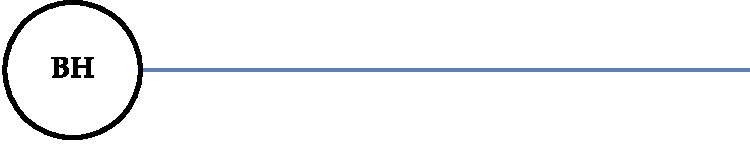
\includegraphics[width=\textwidth]{geodKerr_0_0}
        \caption{ ~$a=0$, ~$L=0$}
    \end{subfigure}
    \hspace{1cm}
    \begin{subfigure}[c]{0.4\textwidth}
        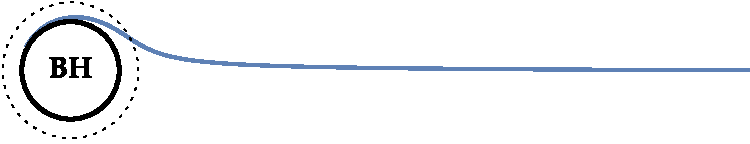
\includegraphics[width=\textwidth]{geodKerr_90_0}
        \caption{~$a=0.9 M$, ~$L=0$}
    \end{subfigure}
    \\
    \vspace{0.3cm}
    \begin{subfigure}[c]{0.4\textwidth}
        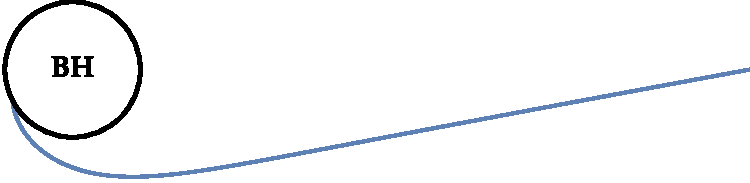
\includegraphics[width=\textwidth]{geodKerr_0_-5}
        \caption{~$a=0$, ~$L<0$}
    \end{subfigure}
    \hspace{1cm}
    \begin{subfigure}[c]{0.4\textwidth}
        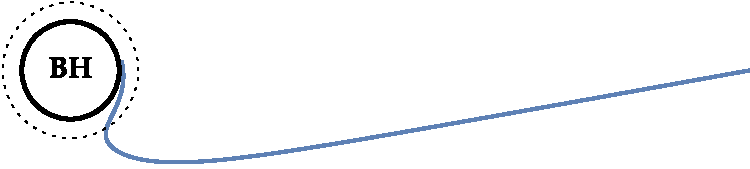
\includegraphics[width=\textwidth]{geodKerr_90_-5}
        \caption{~$a=0.9 M$, ~$L<0$}
    \end{subfigure}
    \caption{Illustration of the Schwarzschild ({\footnotesize\textsc{A,C}}) and Kerr ({\footnotesize\textsc{B,D}}) null equatorial infalling geodesics given by Eqs. \eref{eq2:geodesicTPhi}, for $r(0)=20 M$, with emphasis on $L\ne0$. Even starting with opposite angular momentum, the Kerr geodesic ({\footnotesize\textsc{D}}) is forced to co-rotate with the BH once crossed the ergoregion (dotted).}
    \label{fig2:geodesics}
\end{figure}

Despite BHs being always thought as ``perfect absorbers'' due to the existence of a casual boundary, the ergoregion allows energy extraction from the BH, through the Penrose process, an intrinsic feature of rotating BHs.
Much like spontaneous pair creation and amplification at discontinuities are related but distinct effects, the Penrose process allows for a better understating of the phenomena of superradiance in GR. 

Considering a particle with rest mass $\mu$ and four-momentum $p^\alpha = \mu u^\alpha$, we may identify the constant of motion 
\begin{align}
    E = \bm{k} \cdot \bm{p} = \mu ( g_{tt} p^t + g_{t\varphi} p^\varphi ) ~.
    \label{eq2:PenroseE0}
\end{align}
as it's energy measured by a stationary observer at infinity, due to relations \eref{eq2:geodesicConsts}.
As shown above, the Killing vector is asymptotically timelike but is spacelike inside the ergoregion, thus $g_{tt}<0$.
For a future-directed geodesic, $p^0 = \mu u^0 > 0$, the energy beyond the ergosurface needs not to be positive.
Suppose, that by some means such particle manages to decay inside the ergoregion into two other particles, with momenta $p_1$ and $p_2$. Contracting with $k$, implies that $E = E_1+E_2$. Supposing that the first of the particles has negative energy, $E_1<0$, then 
\begin{align}
    E_2 = E + |E_1| > E ~.
    \label{eq2:PenroseE2}
\end{align}
It can be shown that the particle with negative energy (bounded) must fall into the BH while the other may escape the ergoregion, with greater energy than the particle sent in. 
Energy is conserved by making the BH absorb the particle with negative energy, therefore resulting in a net energy extraction \cite{Townsend1997}.

\begin{figure}[h]
    \centering
    \vspace{0.2cm}
    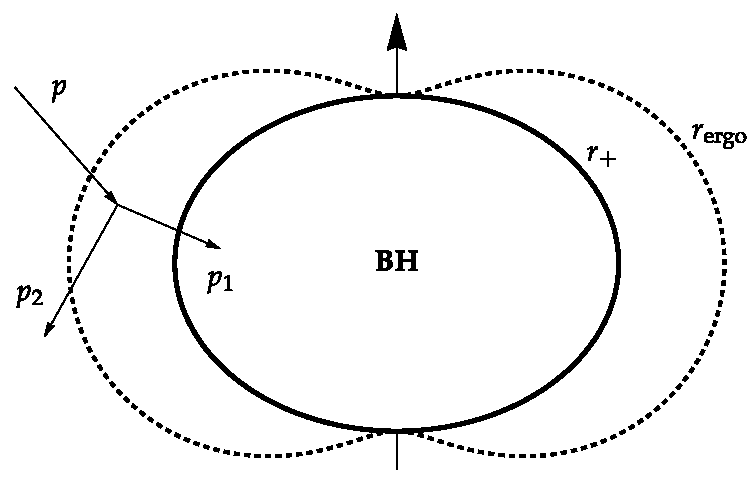
\includegraphics[width=0.65\textwidth]{ergoPenrose}
    \caption{Illustration of the Penrose process, with ergoregion (dotted) and event horizon surfaces parameterized in Kerr-Schild cartesian coordinates.}
    \label{fig2:penroseProcess}
\end{figure}

To understand the limits of the Penrose process, we use the fact that a stationary observer near the horizon must follow orbits of $\bm{\xi}$, given by \eqref{eq2:KillingXi}. 
Although a particle may have negative energy as measured by an asymptotic observer, the stationary one at the horizon must measure a positive energy, as both he and the particle must follow the same orbits, which implies that $\bm{\xi} \cdot  \bm{p_1} \le 0$.
The BH will have a variation of mass $\delta M =E_1$ and angular momentum $\delta J = L_1$, where $L_1 = - \bm{m} \cdot \bm{p_1}$ is the particle's angular momentum. As a result,
\begin{align}
    \label{eq2:penroseCondition}
    \delta J \le \frac{2M\left(M^2+\sqrt{M^4-J^2}\right)}{J} \delta M ~,
\end{align}
which is equivalent to $\delta \left(M^2+\sqrt{M^4-J^2}\right) \ge 0$. This quantity is usually refereed as the ``area'' of the event horizon $A=4\pi(r_+^2+a^2)=8\pi\left(M^2+\sqrt{M^4-J^2}\right)$.
Energy extraction from the Penrose process is limited by the requirement that the horizon area must always increase, which is a special case of the second law of BH mechanics \cite{Hawking1973}. 

We can tie the superradiance process with this particle counterpart using a simple and general argument.
Asymptotically, we may think of waves as a collective of quantum (photons, gravitons, \dots), each carrying $\hbar \omega$ of energy and $\hbar m$ of angular momentum \cite{Bekenstein1973}, where $m$ labels a mode with definite angular momentum.
Therefore, when a given quanta is absorbed, the variation of the BH mass and angular momentum is given by
\begin{align}
    \label{eq2:spinMassRatio}
    \delta J = \frac{m}{\omega} \,\delta M ~.
\end{align}
The condition for superradiance \eref{eq1:superradiance} appears explicitly in the second law of BH mechanics \eref{eq2:penroseCondition}, which guarantees that $\delta M (1 - \Omega_H m /\omega)>0$, \emph{i.e.} confirming energy extraction from the BH when superradiance occurs, while the lack of superradiance increases the mass of the BH.

%----------------------------------------------------------------------------------------

\cleardoublepage